\documentclass[a4,12pt]{article}
	\usepackage[UTF8]{ctex}
	\usepackage{datetime2}% to use \DTMnow
	\usepackage{indentfirst}
		\setlength{\parskip}{5pt}% spacing between paragraphs
		\setlength{\parindent}{20pt}% indentation
	\usepackage{geometry}
		\geometry{tmargin=8mm,bmargin=15mm,lmargin=8mm,rmargin=8mm}
	\usepackage{enumitem}
	\usepackage{hyperref}
	\usepackage{amsmath}
	\usepackage{amssymb}% use mathcal, etc.
	\usepackage{mathtools}
	\usepackage{physics}
	\usepackage{tabu}
	\usepackage{tikz}
		\usetikzlibrary{arrows.meta,calc,decorations.markings,math,arrows.meta,patterns,angles,quotes,decorations.pathreplacing}

% self-defined commands always begin with UPPERCASE LETTER
	\newenvironment{LatinModern}{\fontfamily{lmr}\selectfont}{\par}% Latin Modern
	\DeclareTextFontCommand{\textmyfont}{\LatinModern}
	\newcommand{\Curs}[1]{\emph{\LatinModern{#1}}}
	\newcounter{Problem}
	\newcommand{\Problem}[2]{
		\vspace*{10pt}
		% \stepcounter{Problem}
		\label{Problem #1}
		\noindent#1.\emph{~#2}
	}
	\newcommand{\Qed}{\hfill\ensuremath{\square}}

% useful symbols
	\def\Tick{\ding{51}}
	\newcommand{\rectangle}{{
		\ooalign{$\sqsubset\mkern3mu$\cr$\mkern3mu\sqsupset$\cr}
	}}

\begin{document}

% Title
	\title{
		\vspace*{-50pt}
		\Large{\textbf{太平华联中学数学竞赛题解}\vspace*{-10pt}}\\
	}
	\author{作者:郑其恩 Fanurs\vspace*{-30pt}}
	\date{最后编译时间:\DTMnow (美东)}
	\maketitle
	\vspace*{-25pt}

% \setcounter{Problem}{0}
\Problem{6}{
	由$2, 5, 6$这三个数字所组成的数字不重复的三位数中,其中有几个可以被$3$整除?
	}

	三的整除规则为:若某数的各位数之和为三的倍数,则该数也会是三的倍数;相反的,若某数为三的倍数,则其各位数之和亦可被三整除。

	因此无论我们用$2, 5, 6$组成任何三位数,且数字不重复,比如$256, 562, 625$等,它们的各位数之和皆为
	\[ 2+5+6 = 13 \ \mbox{。} \]
	由于$13$不是$3$的倍数,因此$256, 562, 625$等数都不会被$3$整除。

	因此一共有零个数可以被$3$整除。
	\Qed
	\vspace*{30pt}

	\noindent 点评:
	\begin{enumerate}[label=(\alph*)]
		\item 作者昨日才听说数的整除规则似乎已从新数学课本中剔除,故在此会花多点篇幅讲解之。
		\item 课本没有提及,但网络发达的廿一世纪里,是阻挡不住好学的人。上网搜索“数的整除性”,便可找到许许多多资料。中学竞赛里,至少要熟记$2, 3, 4, 5, 6, 8, 9, 10, 11$的整除规则。
		\item 整除规则的发明(或发现)是为了能不通过“直接相除”,也能百分之百判断出整除性。比如简单的$2$的整除性,只要个位数是$0, 2, 4, 6, 8$其中之一,则该数可被$2$整除,即面对比如像$n=299792458$,我们可通过$2$的整除规则,观察个位数为$8$,从而直接判断$2|n$,即$2$能整除$n$。
		\item 感兴趣的同学可以尝试证明或弄明白为什么这些整除规则成立。作者在此将快速证明下$3$的整除规则。考虑一正整数$n=\overline{a_1a_2\ldots a_k}$,我们想知道此数能否被$3$整除。首先,我们把$n$根据十进制拆解,得
			\[ n = \overline{a_1a_2\ldots a_k} = 10^ka_1 + 10^{k-1}a_2 + \cdots + 10^1a_{k-1} + 10^0a_k \ \mbox{。} \]
			接下来,我们观察到每一项都能进一步拆解,比如$10^ka_1 = (10^k-1)a_1 + a_1$:
			\[ n = [(10^k-1)a_1 + (10^{k-2}-1)a_2 + \cdots + (10^1-1)a_{k-1} + (10^0-1)a_k] + (a_1 + a_2 + \cdots + a_{k-1} + a_k) \ \mbox{。} \]
			现在我们注意到方括号里的每一项其实都是$3$的倍数。为什么?假设$k=3$,则方括号里将变成
			\[ \begin{aligned}
					(1000-1)a_1 + (100-1)a_2 + (10-1)a_3 + (1-1)a_4
					&= 999a_1 + 99a_2 + 9a_3 \\
					&= 3(333a_1 + 33a_2 + 3a_3) \ \mbox{。}
				\end{aligned}
			\]
			事实上,如果学过高阶二项因式分解,我们就会知道$10^k-1=(10-1)(10^{k-1} + 10^{k-2} + \cdots + 10^1 + 10^0)$,所以以上观察对任何正整数$k$都是成立的。因此,如果想知道$n$是否被$3$整除,我们变能直接省略掉方括号里的项(因为他们一定被$3$整除),只需要考虑剩下的$(a_1+a_2+\cdots+a_{k-1}+a_k)$。咦?这不就是各位数之和吗?证毕。
		\item 上述证明中,作者尽可能地保留了式子的一般性\footnote{数学中的“一般性”(generality)其实一点都“不一般”,它是指“(一定条件底下)任意情况都能成立”的意思。生活中,我们说“一般情况”是指大部分会发生的情况,而数学里的“一般情况”却是用来表示某数学定理的“普世性”。}(generality),所以才会有一大堆的“代数符号”。但整个证明的“核心精神”其实是很直观的。我们以$n=46373$为例,想知道$3$是否能整除它。依照上述证明的步骤,但这次有具体的数字为例,我们对$n$进行以下一系列拆解和改写:
			\[ \begin{aligned}
					n
					&= 46373 \\
					&= 10000\times4 + 1000\times6 + 100\times3 + 10\times7 + 1\times3 \\
					&= (9999\times4 + 4) + (999\times6 + 6) + (99\times3 + 3) + (9\times7 + 7) + (3) \\
					&= (9999\times4 + 999\times6 + 99\times3 + 9\times7) + (4 + 6 + 3 + 7 + 3) \\
					&= 3(3333\times4 + 333\times6 + 33\times3 + 3\times7) + (4+6+3+7+3) \ \mbox{。}
				\end{aligned}
			\]
			这时候如果我们把$n\divisionsymbol3$,则有
			\[ \begin{aligned}
					\frac{n}{3}
					&= \frac{3(3333\times4 + 333\times6 + 33\times3 + 3\times7) + (4+6+3+7+3)}{3} \\
					&= \frac{3(3333\times4 + 333\times6 + 33\times3 + 3\times7)}{3} + \frac{(4+6+3+7+3)}{3} \\
					&= (3333\times4 + 333\times6 + 33\times3 + 3\times7) + \frac{(4+6+3+7+3)}{3} \ \mbox{。}
				\end{aligned}
			\]
			由此可见,想知道$n$是否被$3$整除,只需要计算
			\[ \frac{(4+6+3+7+3)}{3} = \frac{23}{3} \ \mbox{。} \]
			因此,$46373$无法被$3$整除。
	\end{enumerate}

\pagebreak
\Problem{3}{
	若四位数$\overline{2x79}$可以被$99$整除,求$x$。
	}

	接上一题,作者假设同学已掌握了$2, 3, 4, 5, 6, 8, 9, 10, 11$的整除规则。

	面对$11$以上的整除规则,通常的做法是把除数因数分解成几个我们已经知道整除规则的数。因此,与其问“四位数$\overline{2x79}$如何才被$99$整除?”,我们可问“四位数$\overline{2x79}$如何才被$9$和$11$同时整除”。这两个问题是等价的。

	先考虑$9$的整除规则:计算各位数之和,其结果能被$9$整除。由此,我们要求$2+x+7+9$是$9$的倍数,故$x=0$或$x=9$。

	接着考虑$11$的整除规则:从高位到低位交错加减,其结果能被$11$整除。由此我们要求$+2-x+7-9$是$11$的倍数(可以是负数)。首先,我们先把式子化简,得
	\[ +2-x+7-9 = -x \ \mbox{。} \]
	因此,我们要求$-x$能被$11$整除。由于$x$必须是介于$0$到$9$的整数(因为$\overline{2x79}$是四位数),所以唯一能满足条件的是$x=0$。

	比较以上两个结论,我们发现$x=0$可同时满足$9$和$11$的整除规则,故$x=0$。
	\Qed
	\vspace*{30pt}

	\noindent 点评:
	\begin{enumerate}[label=(\alph*)]
		\item 这类题目在求得解后,不妨进行验证,以确保答题正确。我们求得$2079$。这个数字挺接近$2100 = 21\times100$,所以我们猜$2079\divisionsymbol99=21$。最后我们试试看:
			\[ 21\times99 = 21\times(100 - 1) = 21\times100 - 21 = 2100 - 21 = 2079 \ \mbox{。} \]
			果然没错。
	\end{enumerate}

\pagebreak
\Problem{8}{
	若$2x$及$\frac{55}{x}$都是正整数,则$x$有几个可能值?
	}

	$2x$若要成为正整数,则$x$必须是正整数,由此:$x=1, 2, 3, \ldots$。

	$\frac{55}{x}$若要成为正整数,则$x$必须能整除$55$,由此:
	\[ x = 55, 11, 5, 1, -1, -5, -11, -55 \ \mbox{。} \]

	因此,若要求$2x$及$\frac{55}{x}$都为正整数,则
	\[ x = 1, 5, 11, 55 \ \mbox{。} \]
	一共有$4$个可能值。
	\Qed
	\vspace*{30pt}

	\noindent 点评:
	\begin{enumerate}[label=(\alph*)]
		\item 这题其实主要就是在问$55$的所有因数。
	\end{enumerate}

\pagebreak
\Problem{10}{
	由$1000000$到$9999999$的整数中,有多少个含有$0, 1, 2, 3, 4, 5, 6$这$7$个数字的每一个各一次?
	}

	$1000000$到$9999999$的整数范围,其实就是所有的七位数。题目的意思就是问有多少个七位数,是由$0, 1, 2, 3, 4, 5, 6$不重复第组成。比如:$6543210, 1023456$等。

	显然,我们不能够把$0$作为数字的开头,因为$0123456$并不是一个数,或者说,不是一个合格的七位数。

	第一格子:从左边算起第一个格子只能摆入$1, 2, 3, 4, 5, 6$这{\color{red}$6$个数字其中之一}。我们就假设先摆入$1$吧!
	\[ \fbox{1}\fbox{?}\fbox{?}\fbox{?}\fbox{?}\fbox{?}\fbox{?} \]
	第二格:剩下$6$个空格,而剩下的数字有$0, 2, 3, 4, 5, 6$。我们须摆入这{\color{red}$6$个数字其中之一},假设摆入$4$吧!
	\[ \fbox{1}\fbox{4}\fbox{?}\fbox{?}\fbox{?}\fbox{?}\fbox{?} \]
	第三格:剩下$5$个空格,而剩下的数字有$0, 2, 3, 5, 6$。我们须摆入这{\color{red}$5$个数字其中之一},假设摆入$0$吧!
	\[ \fbox{1}\fbox{4}\fbox{0}\fbox{?}\fbox{?}\fbox{?}\fbox{?} \]
	第四格:剩下$4$个空格,而剩下的数字有$2, 3, 5, 6$。我们须摆入这{\color{red}$4$个数字其中之一},假设摆入$5$吧!
	\[ \fbox{1}\fbox{4}\fbox{0}\fbox{5}\fbox{?}\fbox{?}\fbox{?} \]
	第五格:剩下$3$个空格,而剩下的数字有$2, 3, 6$。我们须摆入这{\color{red}$3$个数字其中之一},假设摆入$6$吧!
	\[ \fbox{1}\fbox{4}\fbox{0}\fbox{5}\fbox{6}\fbox{?}\fbox{?} \]
	第六格:剩下$2$个空格,而剩下的数字有$2, 3$。我们须摆入这{\color{red}$2$个数字其中之一},假设摆入$2$吧!
	\[ \fbox{1}\fbox{4}\fbox{0}\fbox{5}\fbox{6}\fbox{2}\fbox{?} \]
	第七格:剩下$1$个空格,而剩下的数字有$3$。我们须摆入这{\color{red}$1$个数字其中之一},即$3$。最终得
	\[ \fbox{1}\fbox{4}\fbox{0}\fbox{5}\fbox{6}\fbox{2}\fbox{3} \]

	以上过程中的每一步,依序都分别有{\color{red}$6, 6, 5, 4, 3, 2, 1$}种选择。因此如果我们不断重复上述过程,并且要排出不同的七位数,则一共的排列数有
	$6\times6\times5\times4\times3\times2\times1 = 5040 \ \mbox{。} $
	\Qed
	\vspace*{30pt}

	\noindent 点评:
	\begin{enumerate}[label=(\alph*)]
		\item 初中竞赛遇到组合排列的题目(更深入内容,可见高二的高级数学课本)一般都能通过奇思妙想找出答案。本题把组合一个七位数的过程一步步拆解,然后观察每一步有多少中可能性。最后利用组合排列里的“乘法原理”,把所有可能性相乘得到答案。
		\item 所谓乘法原理,初次听闻的读者可以通过以下例子去直观理解。考虑一个人的穿搭,只考虑上半身的衣服和下半身的裤子。假设这人有$3$件上衣以及$1$条裤子,那显然他只有$3\times1$种选择。而如果另外有一个人有$3$件上衣以及$2$条裤子条裤子,那么可搭配的数量就翻倍,一共有$3\times2$种选择。
	\end{enumerate}

\pagebreak
\Problem{21}{
	下图中,$ABCD$是一梯形,$AB>CD$,$AB\parallel CD$。$M$与$N$分别是线段$AC$与$BD$的中点。若$AB=1024$,$MN=124$,求$CD$的长。
	\begin{center}
	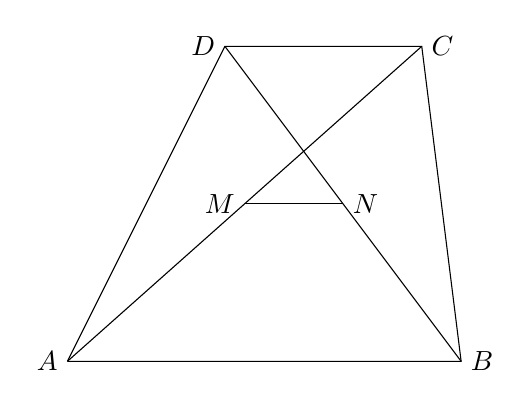
\begin{tikzpicture}
		\coordinate (A) at (0, 0);
		\coordinate (B) at (5, 0);
		\coordinate (C) at (4.5, 4);
		\coordinate (D) at (2, 4);
		\node at (A) [left] {$A$};
		\node at (B) [right] {$B$};
		\node at (C) [right] {$C$};
		\node at (D) [left] {$D$};
		\draw (A)--(B)--(C)--(D)--(A);
		\draw (A)--node[midway, left] (M) {$M$} (C);
		\draw (B)--node[midway, right] (N) {$N$} (D);
		\draw (M)--(N);
	\end{tikzpicture}
	\end{center}
	}

	显然$AC$与$BD$的交点是个重要的点,设之为$O$。
	\begin{center}
	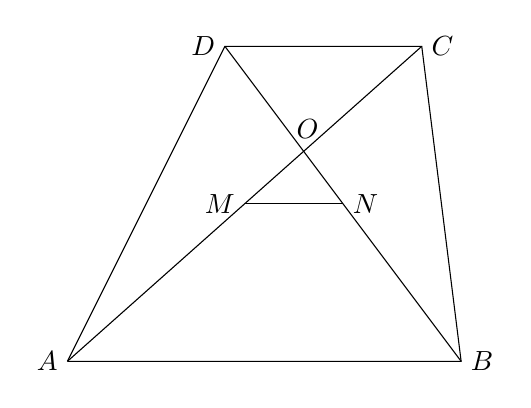
\begin{tikzpicture}
		\coordinate (A) at (0, 0);
		\coordinate (B) at (5, 0);
		\coordinate (C) at (4.5, 4);
		\coordinate (D) at (2, 4);
		\coordinate (O) at (3.05, {3.05*8/9});
		\node at (A) [left] {$A$};
		\node at (B) [right] {$B$};
		\node at (C) [right] {$C$};
		\node at (D) [left] {$D$};
		\node at (O) [above] {$O$};
		\draw (A)--(B)--(C)--(D)--(A);
		\draw (A)--node[midway, left] (M) {$M$} (C);
		\draw (B)--node[midway, right] (N) {$N$} (D);
		\draw (M)--(N);
	\end{tikzpicture}
	\end{center}

	接下来我们需要多次用到相似三角形性质。由于已知$AB$和$MN$的长度,所以我们先从$\triangle{OAB}$和$\triangle{OMN}$开始。首先,因为$M$与$N$分别是线段$AC$与$BD$的中点,所以$MN$比如平行于$AB$和$CD$,即得
	\[ \triangle{OAB}\sim\triangle{OMN} \ \mbox{。} \]
	由于$\triangle{OAB}$相似于$\triangle{OMN}$,所以对应的边比例相等,即
	\[ \frac{AB}{MN} = \frac{AO}{MO} := \lambda \ \mbox{。} \]
	为了方便,我们暂时将$AB:MN$这个比例设为$\lambda$。

	记得,我们的最终目标是找到$CD$,所以一定要想办法跟$\triangle{OCD}$“扯上关系”。再一次,我们根据$MN\parallel CD$,可以推理出
	\[ \triangle{OMN}\sim\triangle{OCD} \ \mbox{。} \]

	有了以上的准备,我们可以开始演算出$CD$了:
	\[ \begin{aligned}
			\frac{AO}{MO} &= \lambda \\
			\frac{AM + MO}{MO} &= \lambda \\
			\frac{CM + MO}{MO} &= \lambda \\
			\frac{(CM - MO) + 2MO}{MO} &= \lambda \\
			\frac{CO + 2MO}{MO} &= \lambda \\
			\frac{CO}{MO} + 2 &= \lambda \\
			\frac{CO}{MO} &= \lambda - 2 \ \mbox{。}
		\end{aligned}
	\]
	最后,根据$\triangle{OMN}\sim\triangle{OCD}$,我们有
	\[ \frac{CD}{MN} = \frac{CO}{MO} = \lambda - 2 \ \mbox{。} \]
	因此
	\[ CD = (\lambda - 2)MN = \left(\frac{AB}{MN} - 2\right)MN = AB - 2MN = 776 \ \mbox{。} \]
	\Qed
	\vspace*{30pt}

	\noindent 点评:
	\begin{enumerate}[label=(\alph*)]
		\item 相似三角形是初中竞赛中最常使用到的知识点之一,也是初中几何的课程范围。参赛同学若正课里还没学过,可以先自己预习或上网观看相关视频。
		\item 好习惯:从最后解答中我们发现其实我们没必要真的算出$\lambda=1024/124$的值,因为最后$(\lambda-2)MN$刚好把分母抵消掉了。所以一个良好的习惯是,先把“已知数字”先设成一个符号,尽可能保留到最后再决定是否需要真的算出来。
	\end{enumerate}

\pagebreak
\Problem{20}{
	下图中,$D$是$AC$上的一点使得$AD=AB$。若$\angle ABC - \angle ACB = 42^\circ$,$\angle CBD = x^\circ$,求$x$。
	\begin{center}
	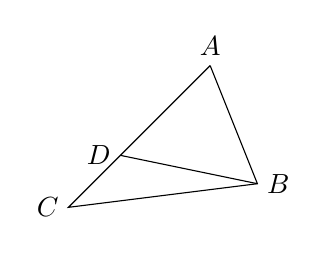
\begin{tikzpicture}[scale=0.6]
		\coordinate (C) at (0, 0);
		\coordinate (B) at (4, 0.5);
		\coordinate (A) at (3, 3);
		\coordinate (D) at (1.1, 1.1);
		\node at (A) [above] {$A$};
		\node at (B) [right] {$B$};
		\node at (C) [left] {$C$};
		\node at (D) [left] {$D$};
		\draw (A)--(B)--(C)--(A);
		\draw (B)--(D);
	\end{tikzpicture}
	\end{center}
	}

	这类题目,在图上把角度写上个代号会很方便。由于$AD=AB$,故$\triangle{ABD}$为等腰三角形,所以$\angle ABD = \angle ADB := s^\circ$。另外我们也设$\angle DAB := r^\circ$及$\angle ACB := t^\circ$。见下图。
	\begin{center}
	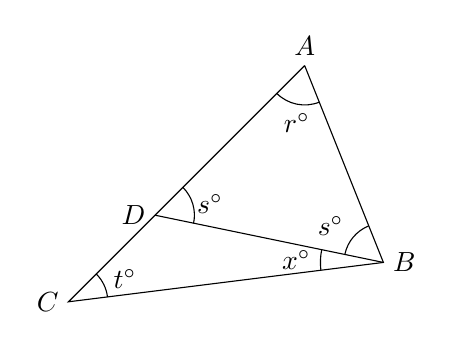
\begin{tikzpicture}
		\coordinate (C) at (0, 0);
		\coordinate (B) at (4, 0.5);
		\coordinate (A) at (3, 3);
		\coordinate (D) at (1.1, 1.1);
		\node at (A) [above] {$A$};
		\node at (B) [right] {$B$};
		\node at (C) [left] {$C$};
		\node at (D) [left] {$D$};
		\draw (A)--(B)--(C)--(A);
		\draw (B)--(D);
		\draw ([shift=(168:0.8)]B) arc(168:187:0.8) node[midway,left] {$x^\circ$};
		\draw ([shift=(-68:0.5)]A) arc(-68:-135:0.5) node[midway,below] {$r^\circ$};
		\draw ([shift=(112:0.5)]B) arc(112:168:0.5) node[midway,left,yshift=4pt] {$s^\circ$};
		\draw ([shift=(-12:0.5)]D) arc(-12:45:0.5) node[midway,right,xshift=-2pt] {$s^\circ$};
		\draw ([shift=(7:0.5)]C) arc(7:45:0.5) node[midway,right,yshift=2pt] {$t^\circ$};
	\end{tikzpicture}
	\end{center}

	有了这些“代号”,题目的已知便可改写如下:
	\[ \begin{aligned}
			\angle ABC - \angle ACB &= 42^\circ \\
			(s+x) - t &= 42 \ \mbox{。}
		\end{aligned}
		\tag{Eq. 1}
	\]
	另外根据三角形内角和为$180^\circ$,从$\triangle{ABD}$及$\triangle{ABC}$分别可得
	\[ 2s + r = 180 \tag{Eq. 2} \]
	及
	\[ (s+x) + r + t = 180 \ \mbox{。} \tag{Eq. 3} \]
	观察发现$\mathrm{(Eq.~1)}+\mathrm{(Eq.~3)}$的左式包含$\mathrm{(Eq.~2)}$的左式,因此
	\[ \begin{aligned}
			[(s+x)-t] + [(s+x)+r+t] &= 42 + 180 \\
			(2s + r) + 2x &= 42 + 180 \\
			180 + 2x &= 42 + 180 \\
			\therefore x &= 21 \ \mbox{。}
		\end{aligned}
	\]
	\Qed
	\vspace*{30pt}

	\noindent 点评:
	\begin{enumerate}[label=(\alph*)]
		\item 本题主要考验“三角形内角和”知识的应用能力和方程求解能力。简单的几何题可通过编写“代号”,让运算变得更简洁而快速。
	\end{enumerate}

\pagebreak
\Problem{12}{
	两支蜡烛,一支红色,一支黄色。它们一样长,且同一时间被点燃。红色蜡烛烧了$6$小时才烧完,黄色蜡烛烧了$3$小时就烧完。若点燃$x$小时后,红色蜡烛的长度是黄色蜡烛的$2$倍,求$60x$的值。
	}

	假设蜡烛长度为$L$,则两支蜡烛的燃烧速度分别为$L/6$(红色)和$L/3$(黄色),而点燃了$x$小时之后的长度分别为$L-(L/6)x$和$L-(L/3)x$。最后根据题目,我们可写出
	\[ \begin{aligned}
			L - \frac{L}{6}x &= 2\left(L - \frac{L}{3}x\right) \\
			1 - \frac{1}{6}x &= 2\left(1 - \frac{1}{3}x\right) \\
			\left(\frac{2}{3} - \frac{1}{6}\right)x &= 2 - 1 \\
			\left(\frac{2}{3} - \frac{1}{6}\right)x &= 2 - 1 \\
			\therefore x &= 2 \ \mbox{。}
		\end{aligned}
	\]
	因此,$60x = 120$。
	\Qed
	\vspace*{30pt}

	\noindent 点评:
	\begin{enumerate}[label=(\alph*)]
		\item 要记得点然后剩下的长度是$L-(L/6)x$,而不是$(L/6)x$。
		\item 记得,速度等于距离除以时间,并以此推导出其他关系式,比如距离等于速度乘以时间。
		\item 其实这题的数字设计得比较小而巧,所以数感不错的同学其实很快就能看到$6-2$恰好是$3-2$的两倍,而蜡烛剩下的长度其实就和要染尽所剩余的时间成比例。
	\end{enumerate}

\pagebreak
\Problem{13}{
	一个课程一共有$n$次考试,已经考了$(n-1)$次。若小明最后一次考试考$100$分,则他在$n$次考试的平均分数是$90$分。若他在最后一次考试考$60$分,则他在$n$次考试的平均分数是$85$分。求$n$的值。
	}

	假设前$(n-1)$次考试的总分为$S$,则根据题目,可列出
	\[ \begin{dcases}
			\frac{S+100}{n} = 90 \\
			\frac{S+60}{n} = 85
		\end{dcases}
		\ \mbox{。}
	\]
	由此可得
	\[ \begin{dcases}
			S + 100 = 90n\\
			S + 60 = 85n
		\end{dcases}
		\ \mbox{。}
	\]
	两式相减后得
	\[ \begin{aligned}
			(S+100) - (S+60) &= 90n - 85n \\
			5n &= 40 \\
			\therefore n &= 8 \ \mbox{。}
		\end{aligned}
	\]
	\Qed
	\vspace*{30pt}

	\noindent 点评:
	\begin{enumerate}[label=(\alph*)]
		\item 作者最近才知道二元一次联立方程式是初二数学下半年的课程,但这在竞赛中是属于比较基本的代数知识了。
		\item 参赛同学如果熟悉了一元一次方程,可以先自习二元一次联立方程式的内容。网上有许多资源,比如:
			\begin{center}\href{https://www.youtube.com/watch?v=x6MhCsllVP0}{https://www.youtube.com/watch?v=x6MhCsllVP0}\end{center}
		\item 其实二元一次方程的主要技巧就是两个(甚至更多)方程式,互相可以加减。只要加减过程中能成果抵消掉其中一个未知数,比如这题里的$S$便通过相减后消失了,那剩下的方程就只有一个未知数$n$,“退化”为一元一次方程式。
	\end{enumerate}

\pagebreak
\Problem{14}{
	一间珠宝店所卖的每粒宝石的价格都是整数,它们的价格在每周一开始就调整。在这个星期,一粒红宝石与一粒蓝宝石的价格一样。红宝石这星期的价格比上星期的上涨了$10\%$,蓝宝石这星期的价格比上星期的下跌了$10\%$。求蓝宝石上星期的价格的最小可能值。
	}

	显然这是一题代数题。

	设上周红蓝宝石的价格分别为$x$和$y$,再根据题目对价格变化的描述,得出
	\[ \begin{aligned}
			110\%\times x &= 90\%\times y \\
			1.1x &= 0.9y \ \mbox{。}
		\end{aligned}
	\]
	到目前位置,方程有无限个解。但是我们有另外一个条件还没用上,那就是“每粒宝石的价格都是整数”。虽然题目没说,但是价格应该也是正数,所以不考虑负数。

	当$x$和$y$被局限于正整数范围,这题目其实就变成了“数论题”,因此我们把方程改写为
	\[ \frac{x}{y} = \frac{9}{11} \ \mbox{。} \]
	显然,一个最直接的解就是$x=9$,$y=11$。这价格还可能更大,比如$(x, y) = (18, 22), (27, 33), \ldots$。但是由于$9$和$11$为质数,所以$(x, y) = (9, 11)$是最小的解了。

	答,蓝宝石上星期的价格的最小可能值为$11$。
	\Qed
	\vspace*{30pt}

	\noindent 点评:
	\begin{enumerate}[label=(\alph*)]
		\item 应用题其实考的就是一点:如何把文字的描述转化为方程式。一旦写成了方程式,我们就能把它转化为我们熟悉的东西(假设你学过),然后求解。这也是数学能在各领域得到广泛应用的主要原因。
		\item 所谓“数论题”就是问“因数”、“整除性”、“质数”等的问题。数论的研究对象一般局限在整数(有时还只考虑正整数),而代数题目一般允许未知数为任意实数(允许小数点)。在初中阶段或许看不出,但数论一直都是几百年来纯数学里的“皇冠”,因为它的问题几乎没太多实际应用(是最纯的数学领域),但却极奇困难,于是吸引了每个时代最顶尖数学家的挑战,也是业余数学爱好者最喜欢的内容。
	\end{enumerate}

\end{document}
